\documentclass[11pt,mathserif]{beamer}

%% ====== packages ==
\usepackage{amsmath,amssymb,amsfonts,amsthm}
\usepackage{graphicx}
\usepackage{bbding}
\newcommand{\tiret}{\rule[0.6ex]{1.3ex}{0.22ex}}

% !! pour le francais
\usepackage[utf8]{inputenc}
\usepackage[french]{babel}
\usepackage{fancyvrb}
%\usepackage{verbatim}
\usepackage{relsize}
\usepackage{color}
\usepackage{listings}

\definecolor{dkgreen}{rgb}{0,0.6,0}
\definecolor{gray}{rgb}{0.5,0.5,0.5}
\definecolor{mauve}{rgb}{0.58,0,0.82}
\definecolor{bleuSympa}{rgb}{0.,0.19,0.607}

\newcommand{\R}{\mathbb{R}}
\lstset{ %
  numbers=left,
  numbersep=1pt,
  numberstyle=\relsize{-5}\ttfamily,
  language=C,                % the language of the code
  framerule=1pt,
  basicstyle=\relsize{-3}\ttfamily,           % the size of the fonts that are used for the code
                                  % will be numbered
  %numbersep=5pt,                  % how far the line-numbers are from the code
  backgroundcolor=\color{black!50},      % choose the background color. You must add \usepackage{color}
  showspaces=false,               % show spaces adding particular underscores
  showstringspaces=false,         % underline spaces within strings
  showtabs=false,                 % show tabs within strings adding particular underscores
  %frame=single,                   % adds a frame around the code
  rulecolor=\color{black},        % if not set, the frame-color may be changed on line-breaks within not-black text (e.g. commens (green here))
  %tabsize=2,                      % sets default tabsize to 2 spaces
  breaklines=true,                % sets automatic line breaking
  breakatwhitespace=false,        % sets if automatic breaks should only happen at whitespace
  lineskip=-1pt,
  keywordstyle=\color{bleuSympa}\textbf,          % keyword style
  commentstyle=\color{dkgreen},       % comment style
  stringstyle=\color{mauve},
  emph={ __global__, __shared__, __device__, __host__,
        __syncthreads, threadIdx},
  emphstyle=\color{green},
  moredelim=[s][\color{green}\ttfamily]{<<<}{>>>},
  morecomment=[s][\color{mauve}]{cudaMemcpyHostToDevice}{\ },
  morecomment=[s][\color{mauve}]{cudaMemcpyDeviceToHost}{\ }
}


% et la commande Pour les guillemets
\newcommand{\guill}[1]{«#1»} % attention deja dans mycv
\defbeamertemplate{itemize item}{boldarrow}{\raisebox{0.3ex}{\resizebox{1.2ex}{1ex}{\ArrowBoldRightShort}}}

%% ====== my bearmer ==
\mode<presentation> {
\usetheme{default}    % sobre

% options
\useinnertheme[shadow]{rounded}  % les numeros
}
\usefonttheme{structurebold}

\begin{document}

%****************************************************************
% Page de presentation 
%**************************************************************
\begin{frame}
\begin{center}
{\Large Une introduction au calcul sur GPU} 
\end{center}
\begin{center}
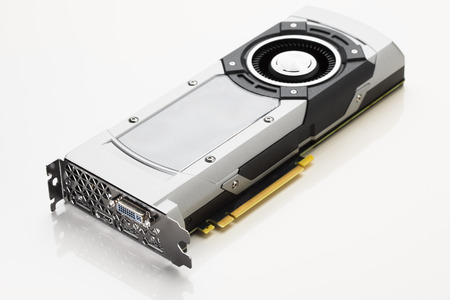
\includegraphics[width=0.5\linewidth]{gpu.jpg}
\end{center}
\begin{center}
{\large Marc Fuentes - INRIA Pau\\ }
\end{center}
\end{frame}

%****************************************************************
% Plan
%**************************************************************

\begin{frame}
\frametitle{Plan}

\begin{itemize}[<+->]
\item Prolégomenes( parallèlisme, mémoire, cache)
\item Architecture des GPU
\item CUDA
\end{itemize}
\end{frame}

%****************************************************************
% Prolegomènes I
%****************************************************************
\begin{frame}
\frametitle{Parallèlisme}
\pause
différentes classifications du parallèlisme
\begin{itemize}[<+->]
  \item partagé / distribué
    \begin{itemize}
      \item à mémoire partagée : OpenMP, fils d'éxecution (Threads), GPU 
      \item à mémoire distribué : MPI, Coarrays Fortran, PGAS
    \end{itemize}
 \item gros grain / grain fin : taille des tâches
   \begin{itemize}
     \item gros grain : MPI, certains tâches en mémoire partagée
     \item grain fin : noyau GPU s'executant sur beaucoup de cœurs
   \end{itemize}
 \item homogène / hétérogène 
   \begin{itemize}
     \item archi homogène : MPI, processeur vectoriels
     \item archi hétérogène : accélérateur vs hôte, Cell 
   \end{itemize}
\end{itemize}
\pause
  $\Rightarrow$ La programmation sur GPU est {\it grosso modo } donc un parallèlisme à {\bf grain fin}, à{\bf mémoire partagée} tournant sur 
  {\bf une archi hétérogène}.
\end{frame}

%****************************************************************
% Prolègomène II
%****************************************************************
\begin{frame}{Mémoire et Cache}
\begin{itemize}[<+->]
  \item La rapidité d'execution d'un calcul dépend aussi de la «proximité» avec le CPU de l'élément de mémoire à traiter 
  \item[$\Rightarrow$] les concepteurs de CPU ont crée des {\bf caches} pour stocker les valeurs mémoires les plus utilisées
  \begin{center}
    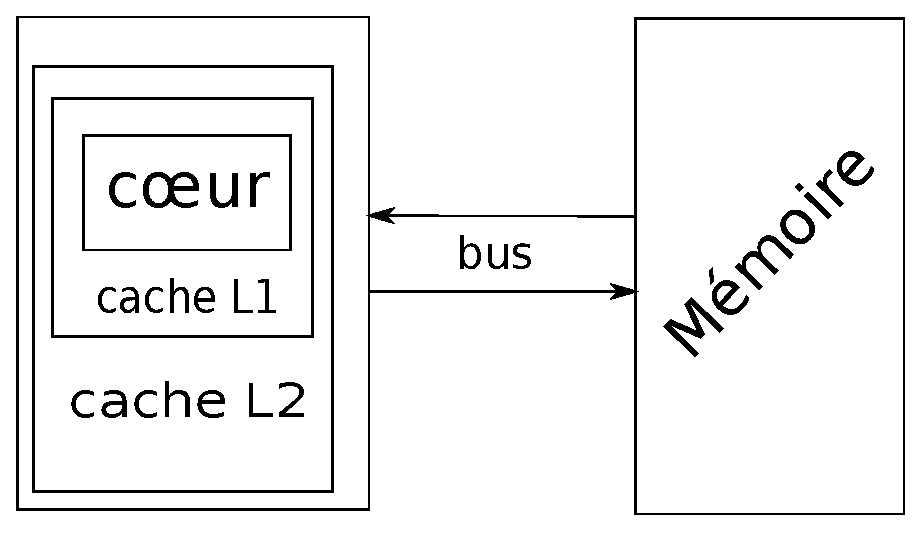
\includegraphics[width=0.7\linewidth]{cpu_classique.eps}
  \end{center}
\end{itemize}
\end{frame}
%****************************************************************
% Prolegomenes III
%****************************************************************
\begin{frame}{Mémoire et Cache II}
\pause
  \begin{itemize}[<+->]
  \item ainsi la latence $l$ de l'emplacement mémoire auquel on accède  respecte
  $$l({\mbox{\scriptsize registre}}) \leqslant l(\mbox{\scriptsize cache L1}) \leqslant
    l(\mbox{\scriptsize cache L2}) \leqslant l(\mbox{\scriptsize mémoire globale}).$$
  \item ordres de grandeur des latences (core i7 Xeon E5500)
    \begin{tabular}{|l|c|c|}
    \hline
      type & nb cycles & latence (ns)  \\
    \hline
      cache L1  &  4 & 2 \\
      cache L2  &  10 & 5 \\
      cache L3 (non partagé) & 40 & 20  \\
      cache L3 (partagé) &  65 & 35  \\
      mémoire vive local & & 60 \\
      mémoire vive distante & & 100 \\
    \hline
    \end{tabular}
  \end{itemize}
\end{frame}
%%****************************************************************
%% Prolegomenes IV
%%****************************************************************
\begin{frame}{Cache : Succés et défauts}
\begin{itemize}[<+->]
 \item succés (hit): accès a un emplacement présent dans la ligne de cache 
 \item défaut (miss) : accès hors de ligne de cache $\rightarrow$ il faut recharger entierement la ligne des cache!
 \item un code localisant les accés dans le cache, va minimiser les défauts de cache et tourner plus vite
 \item double boucle en C sur les lignes (resp. colonnes en Fortran)
\end{itemize}
\pause
\begin{minipage}[c]{0.49\linewidth}
  \lstinputlisting[language=C]{loop_col.c}
\end{minipage}
\begin{minipage}[c]{0.49\linewidth}
    \begin{tabular}{|c|c|}
    \hline
     boucle ext. & tps(s)  \\
    \hline
      i (lignes) & 2.7s \\
      j (cols)  & 3.4s \\
    \hline
    \end{tabular}
\end{minipage}
\pause 
 $\Rightarrow$ raison d'être des biblios BLAS et LAPACK
\end{frame}
%%****************************************************************
%% Prolegomenes V
%%****************************************************************
\begin{frame}{Passage à l'echelle}
\begin{itemize}[<+->]
  \item Fort (strong scalability)
    \begin{itemize} 
       \item loi d'Amdhal (pessimiste)
    \end{itemize}
  \item faible (weak scalability)
    \begin{itemize}
      \item loi
    \end{itemize}
\end{itemize}
\end{frame}
%%****************************************************************
%% Exemple introductif I
%%****************************************************************
\begin{frame}{Exemple d'introduction (I)}
\pause
\begin{itemize}[<+->]
 \item considerons le programme simplifié suivant
\lstinputlisting{increment.c}
\item on souhaite paralléliser la boucle en ligne 6 à l'aide de CUDA
\end{itemize}
\end{frame}
%%****************************************************************
%% Exemple introductif II
%%****************************************************************
\begin{frame}{Exemple d'introduction II }
\pause
\begin{itemize}[<+->]
 \item on peut écrire le programme suivant
\lstinputlisting{incrementGPU.cu}
\item plus de boucle!
\item nouveaux mot-clef : \texttt{\_\_global\_\_, threadIdx}
\item appel du noyau \texttt{increment<<<1,N>>>}
\item gestion de la mémoire : \texttt{cudaMemcpy, cudaMalloc, cudaFree}
\end{itemize}
\end{frame}
\end{document}

